
\begin{enumerate}[\bfseries 1.]

    %------------------- ley asociativa --------------------
    \item \textbf{Mostrar gráficamente la ley asociativa.\\\\
	Repuesta.-}\; Sea los vectores $\vec{a},\vec{b}$ y $\vec{c}\in V_n$, entonces:
	\begin{center}
	    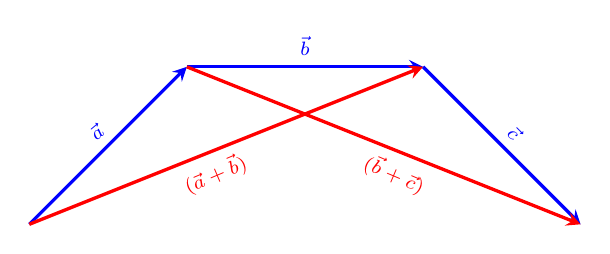
\begin{tikzpicture}[scale=2]
		\tikzstyle{every node}=[font=\scriptsize]
		\draw[line width=1.2pt,blue,-stealth](0,0)--(1,1) node[rotate=40,pos=0.5,above]{$\vec{a}$};
	      \draw[line width=1.2pt,blue,-stealth](1,1)--(2.5,1) node[pos=0.5, above]{$\vec{b}$};
	      \draw[line width=1.2pt,blue,-stealth](2.5,1)--(3.5,0) node[rotate=-45,pos=0.5, above]{$\vec{c}$};
	      \draw[line width=1.2pt,red,-stealth](1,1)--(3.5,0) node[rotate=-23,pos=0.55, below]{$(\vec{b}+\vec{c})$};
	      \draw[line width=1.2pt,red,-stealth](0,0)--(2.5,1) node[rotate=23,pos=0.45, below]{$(\vec{a}+\vec{b})$};
	    \end{tikzpicture}
	\end{center}
	De donde podemos deducir que:
	$$\vec{a}+\left(\vec{b}+\vec{c}\right)=\left(\vec{a}+\vec{b}\right)+\vec{c}.$$\\

    %------------------- Angulo --------------------
    \item \textbf{\boldmath Demuestre que $\alpha=30^\circ$.\\\\
	Respuesta.-}\; Demostremos gráficamente:
	\begin{center}
	    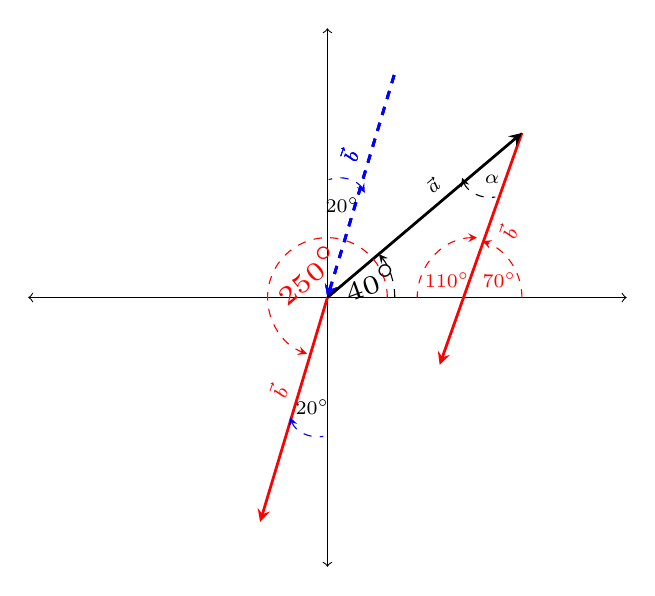
\begin{tikzpicture}[scale=1.9]
		\tikzstyle{every node}=[font=\scriptsize]
		\draw[<->] (-2,0)--(2,0);
		\draw[<->] (0,-1.8)--(0,1.8);
		\draw[line width=1pt,red,-stealth](0,0)--(-.45,-1.5) node[rotate=70,pos=0.45, above]{$\vec{b}$};
		\draw[dashed,line width=1pt,blue,stealth-](0,0)--(.45,1.5) node[rotate=70,pos=0.6, above]{$\vec{b}$};
		\draw[dashed,line width=1pt,blue,stealth-](0,0)--(.45,1.5) node[rotate=70,pos=0.6, above]{$\vec{b}$};
		\draw[line width=1pt,red,stealth-](.75,-.45)--(1.3,1.1) node[rotate=70,pos=0.6, below]{$\vec{b}$};
		\draw[dashed,line width=1pt,blue,stealth-](0,0)--(.45,1.5) node[rotate=70,pos=0.6, above]{$\vec{b}$};
		\draw[line width=1pt,-stealth](0,0)--(1.3,1.1) node[rotate=40,pos=0.6, above]{$\vec{a}$};
		\draw[red,dashed,-stealth](.4,0)node[pos=0.5,rotate=40,above]{\tiny$250^\circ$} arc (0:250:.4);
		\draw[dashed,-stealth](.45,0)node[pos=1,rotate=20,right]{\tiny$40^\circ$} arc (0:40:.45);
		\draw[red,dashed,-stealth](1.3,0) arc (0:70:.4);
		\draw[red](1.15,0)node[above]{$70^\circ$};
		\draw[red,dashed,stealth-](1,0.4) arc (90:180:.4);
		\draw[red](.8,0)node[above]{$110^\circ$};
		\draw[dashed,stealth-](.9,0.8) arc (200:280:.2);
		\draw[](1.1,.7)node[above]{$\alpha$};
		\draw[blue,dashed,stealth-](-.25,-0.8) arc (200:280:.2);
		\draw[](-.1,-.85)node[above]{$20^\circ$};
		\draw[blue,dashed,stealth-](.25,0.7) arc (30:110:.2);
		\draw[](.1,.5)node[above]{$20^\circ$};
	    \end{tikzpicture}
	\end{center}

	Ya que los ángulos internos de un triángulo forman $180^\circ$ entonces,
	$$180^\circ = 110^\circ +40^\circ + \alpha \quad \Rightarrow \quad \alpha=30^\circ.$$\\
	
	

\end{enumerate}
